
\begin{figure}[H]
\begin{center}
\subfloat{
\resizebox{8cm}{5cm}{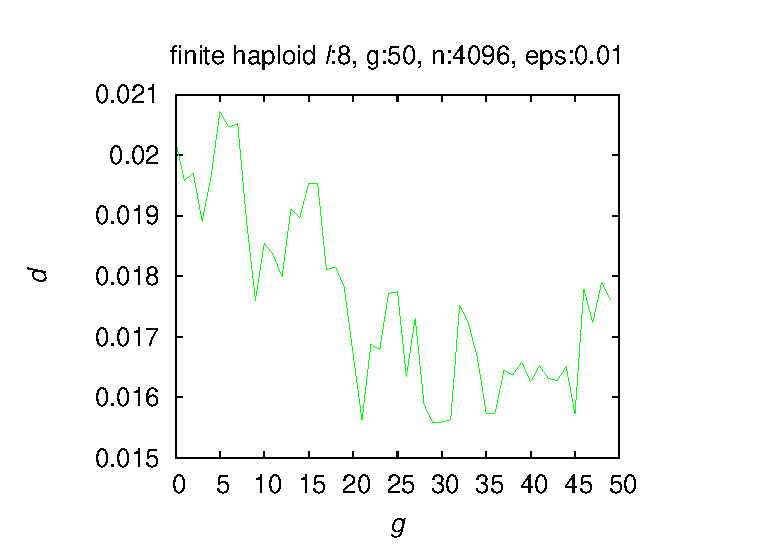
\includegraphics{figures/eps/vio/mu/b8/e0.01/n00004096_fin_hap.eps}}} \hspace{-3em}%
\subfloat{
\resizebox{8cm}{5cm}{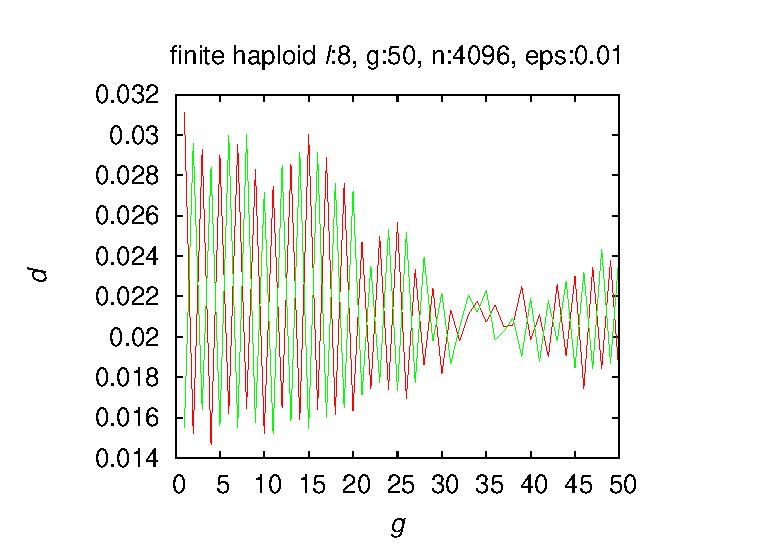
\includegraphics{figures/eps/vio/mu/b8/e0.01/n00004096_fin_hap_wovio.eps}}}\vspace{-1em} \hspace{-3em}%
\end{center}
\begin{center}
\subfloat{
\resizebox{8cm}{5cm}{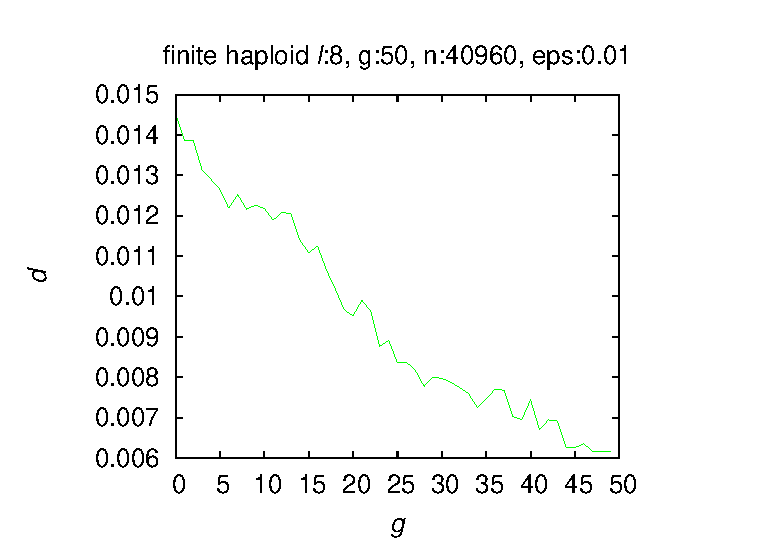
\includegraphics{figures/eps/vio/mu/b8/e0.01/n00040960_fin_hap.eps}}} \hspace{-3em}%
\subfloat{
\resizebox{8cm}{5cm}{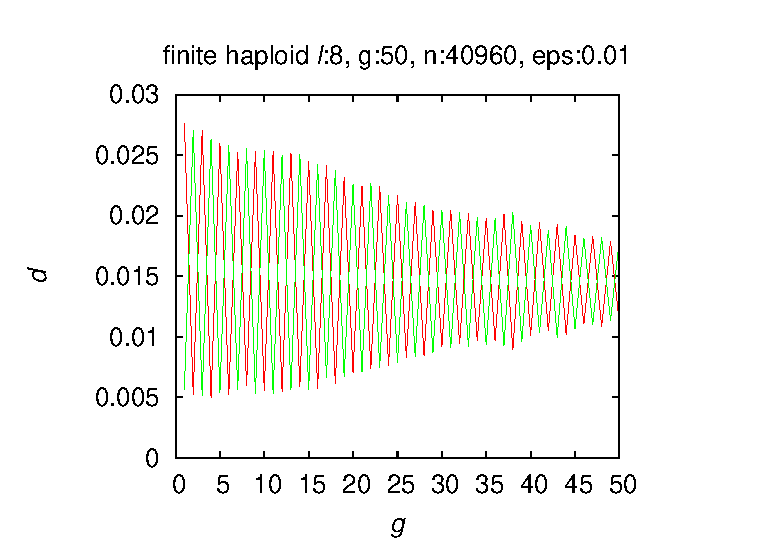
\includegraphics{figures/eps/vio/mu/b8/e0.01/n00040960_fin_hap_wovio.eps}}}\vspace{-1em} \hspace{-3em}%
\end{center}

\begin{center}
\subfloat{
\resizebox{8cm}{5cm}{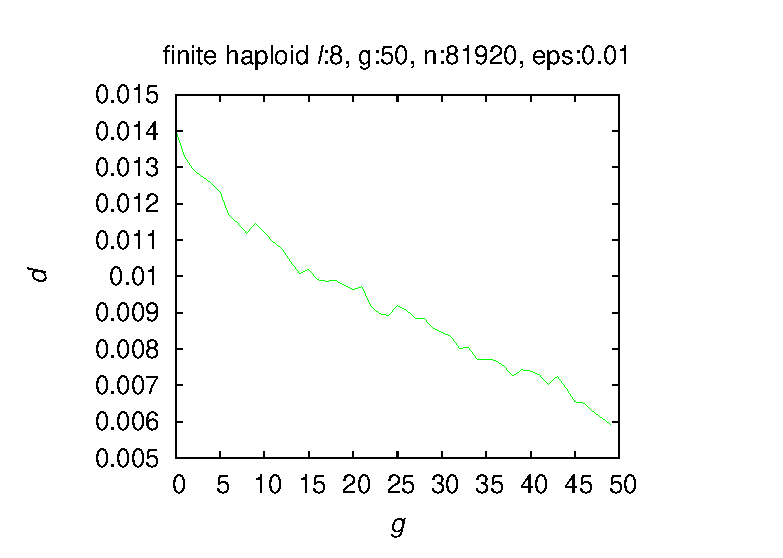
\includegraphics{figures/eps/vio/mu/b8/e0.01/n00081920_fin_hap.eps}}} \hspace{-3em}%
\subfloat{
\resizebox{8cm}{5cm}{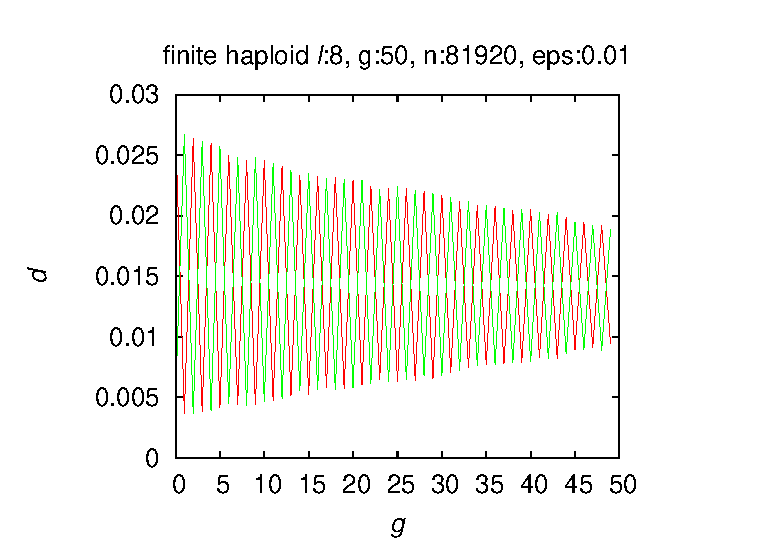
\includegraphics{figures/eps/vio/mu/b8/e0.01/n00081920_fin_hap_wovio.eps}}}\vspace{-1em} \hspace{-3em}%
\end{center}

\begin{center}
\subfloat{
\resizebox{8cm}{5cm}{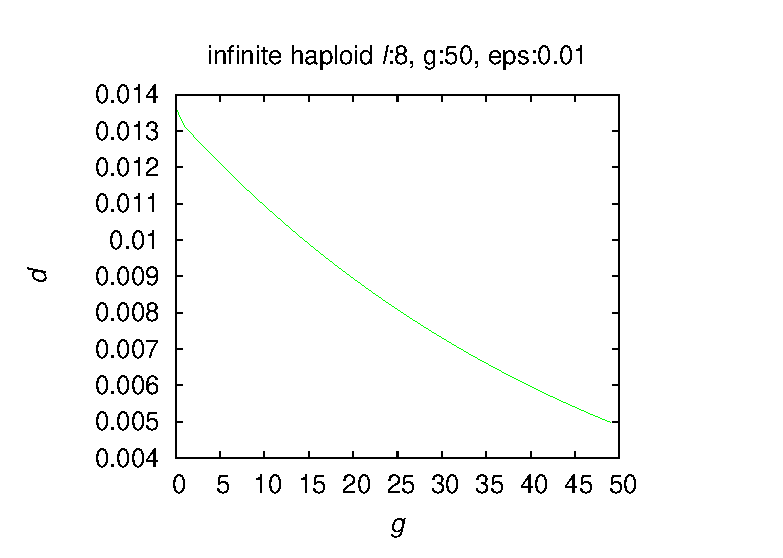
\includegraphics{figures/eps/vio/mu/b8/e0.01/inf_hap.eps}}}\hspace{-3em}%
\subfloat{
\resizebox{8cm}{5cm}{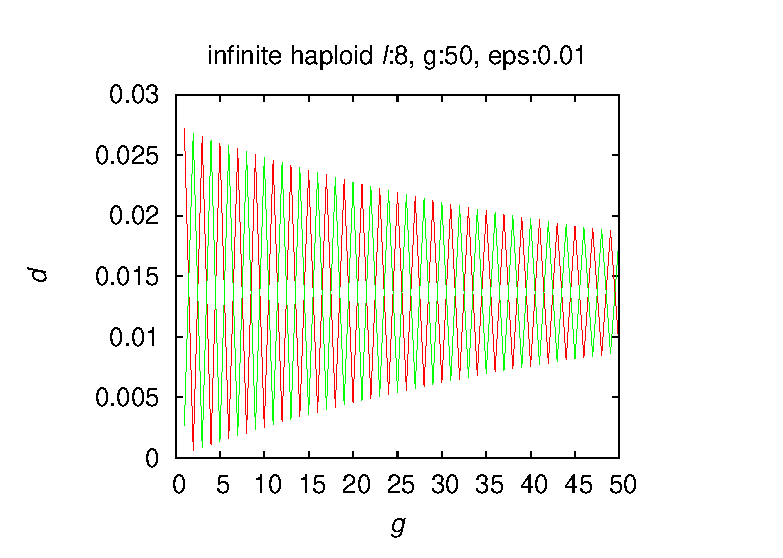
\includegraphics{figures/eps/vio/mu/b8/e0.01/inf_hap_wovio.eps}}}\vspace{-0.5em} \hspace{-3em}%


\caption{\textbf{Infinite and finite haploid population oscillation behavior in case of violation in $\bm{\mu}$ for genome length $\ell = 8$ and $\epsilon = 0.01$:} 
  In left column, $d$ is distance of finite population of size $n$ or infinite population to limit for $g$ generations. In right column, $d$ is distance of finite population of size $N$ or infinite population to limits without violation.}
\label{oscillation_8h_vio_mu_0.01}
\end{center}
\end{figure}

\begin{figure}[H]
\begin{center}
\subfloat{
\resizebox{8cm}{5cm}{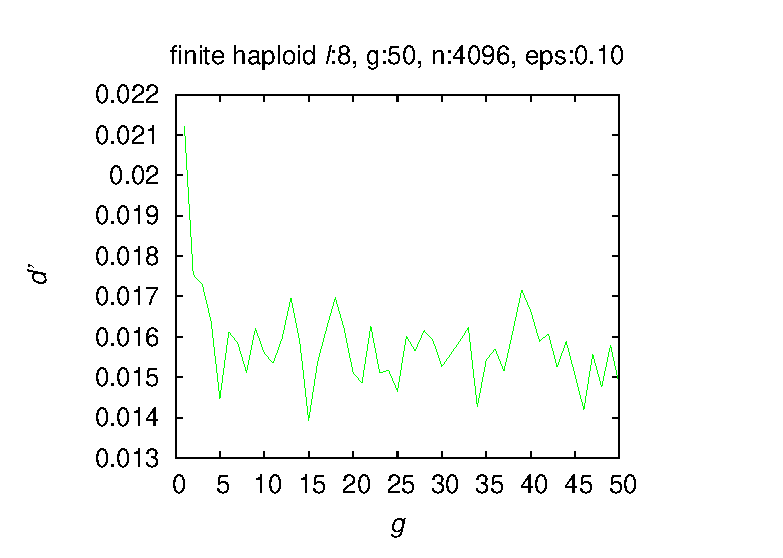
\includegraphics{figures/eps/vio/mu/b8/e0.1/n00004096_fin_hap.eps}}}  \hspace{-3em}%
\subfloat{
\resizebox{8cm}{5cm}{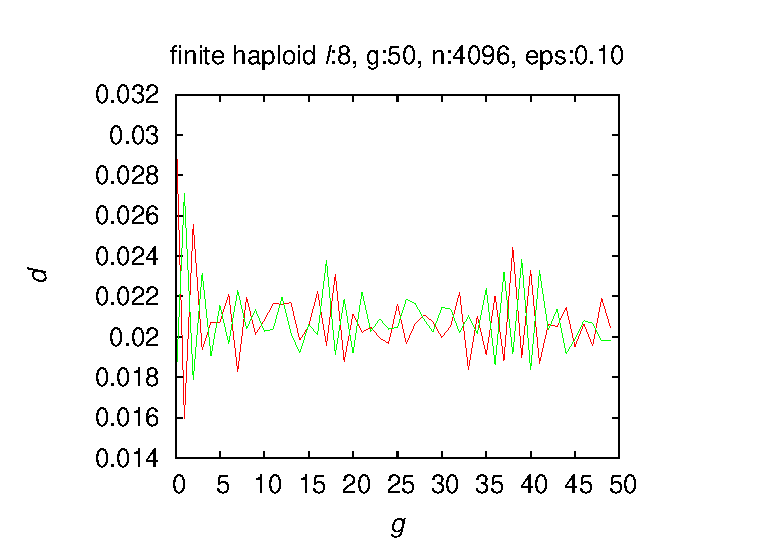
\includegraphics{figures/eps/vio/mu/b8/e0.1/n00004096_fin_hap_wovio.eps}}}\vspace{-1em}  \hspace{-3em}%
\end{center}
\begin{center}
\subfloat{
\resizebox{8cm}{5cm}{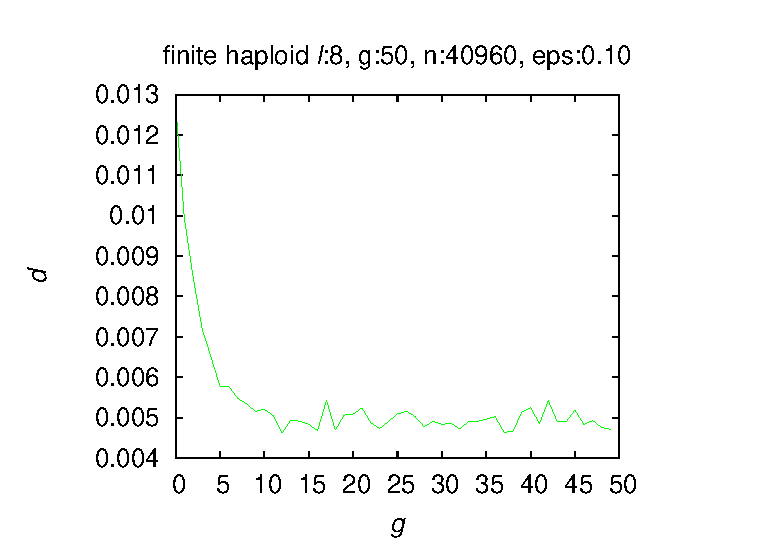
\includegraphics{figures/eps/vio/mu/b8/e0.1/n00040960_fin_hap.eps}}}  \hspace{-3em}%
\subfloat{
\resizebox{8cm}{5cm}{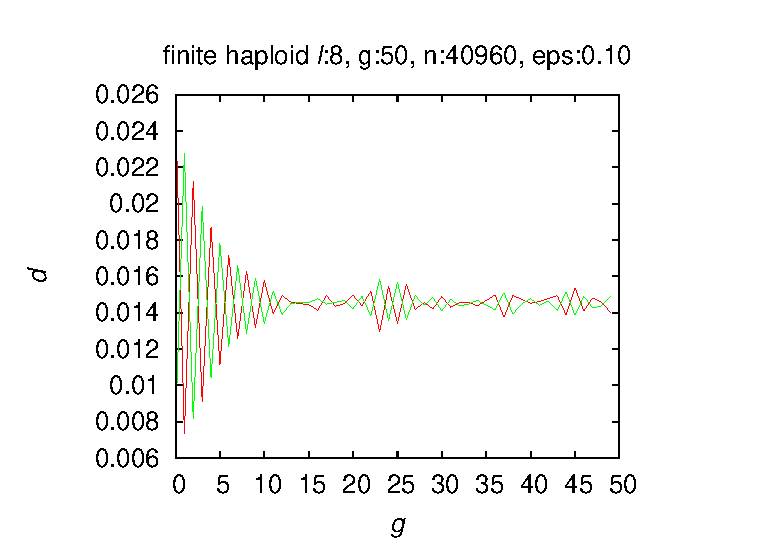
\includegraphics{figures/eps/vio/mu/b8/e0.1/n00040960_fin_hap_wovio.eps}}}\vspace{-1em}  \hspace{-3em}%
\end{center}

\begin{center}
\subfloat{
\resizebox{8cm}{5cm}{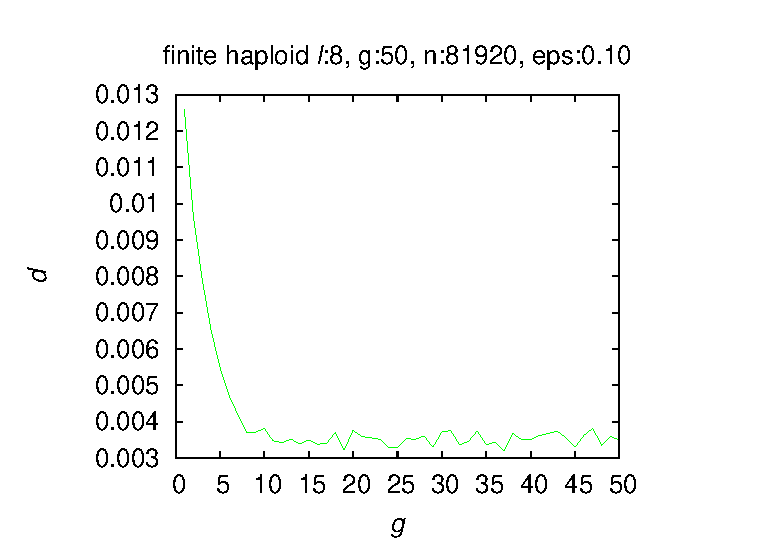
\includegraphics{figures/eps/vio/mu/b8/e0.1/n00081920_fin_hap.eps}}}  \hspace{-3em}%
\subfloat{
\resizebox{8cm}{5cm}{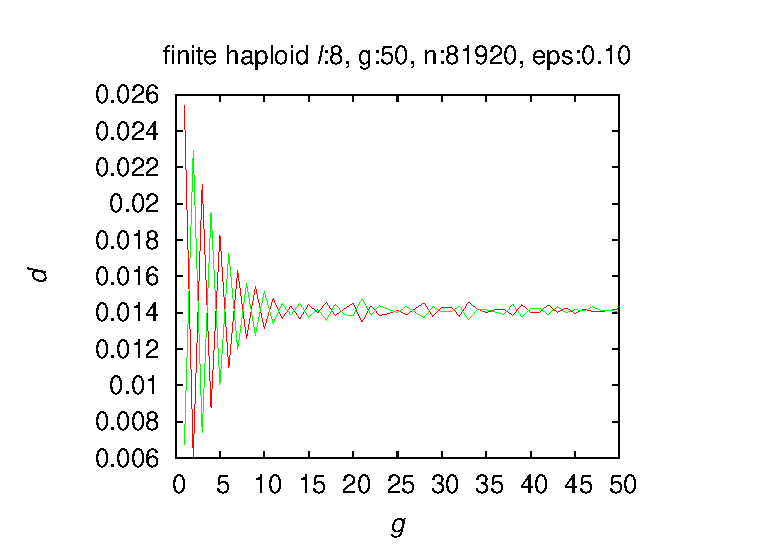
\includegraphics{figures/eps/vio/mu/b8/e0.1/n00081920_fin_hap_wovio.eps}}}\vspace{-1em}  \hspace{-3em}%
\end{center}

\begin{center}
\subfloat{
\resizebox{8cm}{5cm}{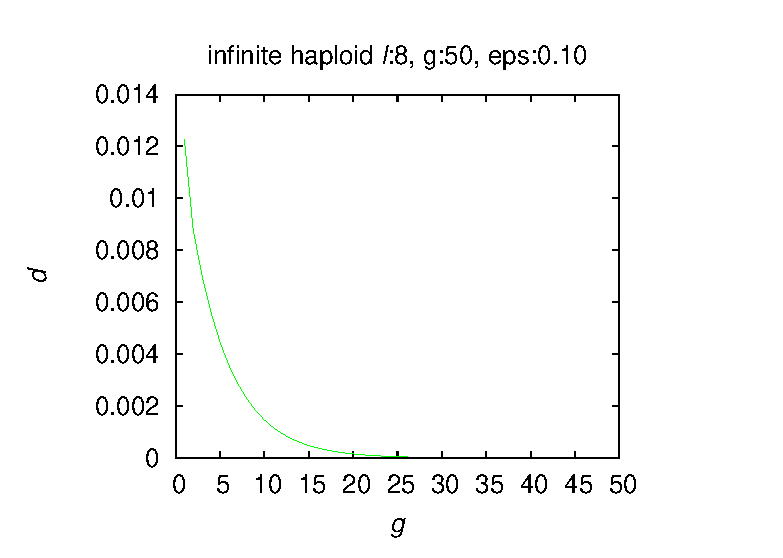
\includegraphics{figures/eps/vio/mu/b8/e0.1/inf_hap.eps}}} \hspace{-3em}%
\subfloat{
\resizebox{8cm}{5cm}{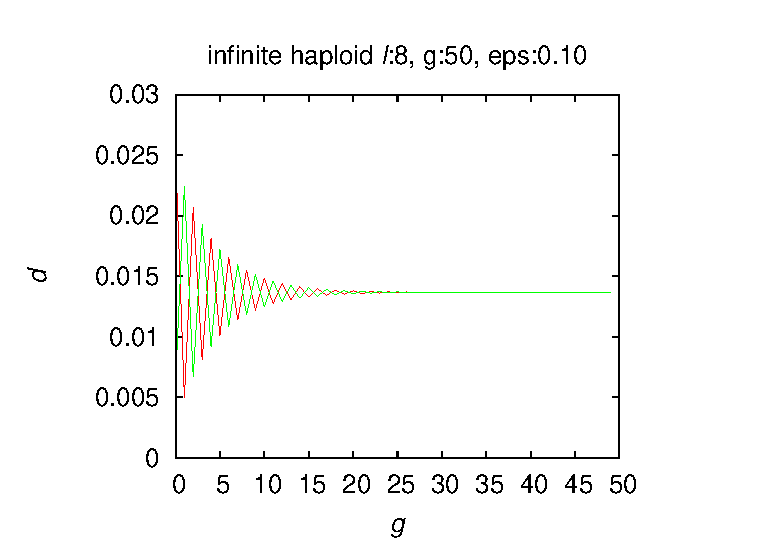
\includegraphics{figures/eps/vio/mu/b8/e0.1/inf_hap_wovio.eps}}}\vspace{-0.5em}  \hspace{-3em}%


\caption{\textbf{Infinite and finite haploid population oscillation behavior in case of violation in $\bm{\mu}$ for genome length $\ell = 8$ and $\epsilon = 0.1$:} 
  In left column, $d$ is distance of finite population of size $n$ or infinite population to limit for $g$ generations. In right column, $d$ is distance of finite population of size $N$ or infinite population to limits without violation.}
\label{oscillation_8h_vio_mu_0.1}
\end{center}
\end{figure}


\begin{figure}[H]

\begin{center}
\subfloat{
\resizebox{8cm}{5cm}{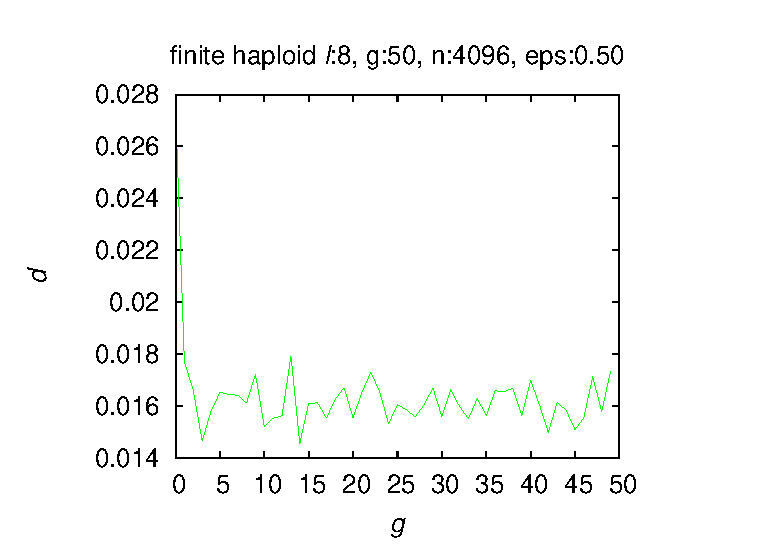
\includegraphics{figures/eps/vio/mu/b8/e0.5/n00004096_fin_hap.eps}}}  \hspace{-3em}%
\subfloat{
\resizebox{8cm}{5cm}{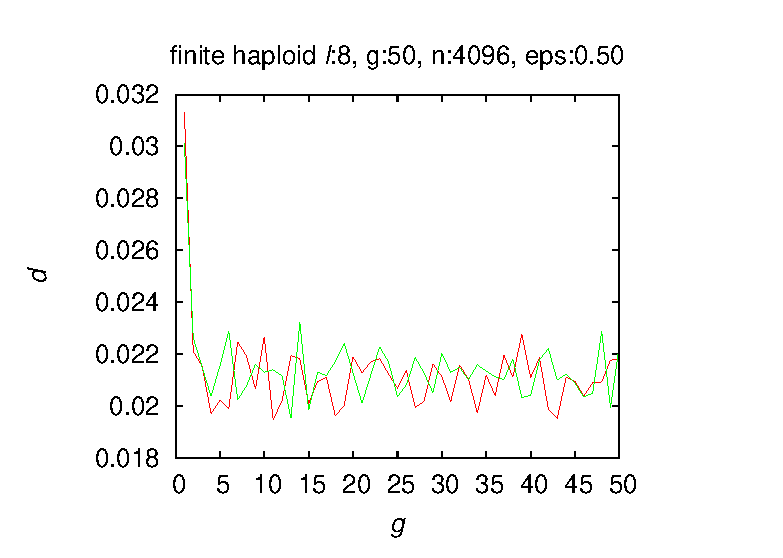
\includegraphics{figures/eps/vio/mu/b8/e0.5/n00004096_fin_hap_wovio.eps}}}\vspace{-1em}  \hspace{-3em}%
\end{center}
\begin{center}
\subfloat{
\resizebox{8cm}{5cm}{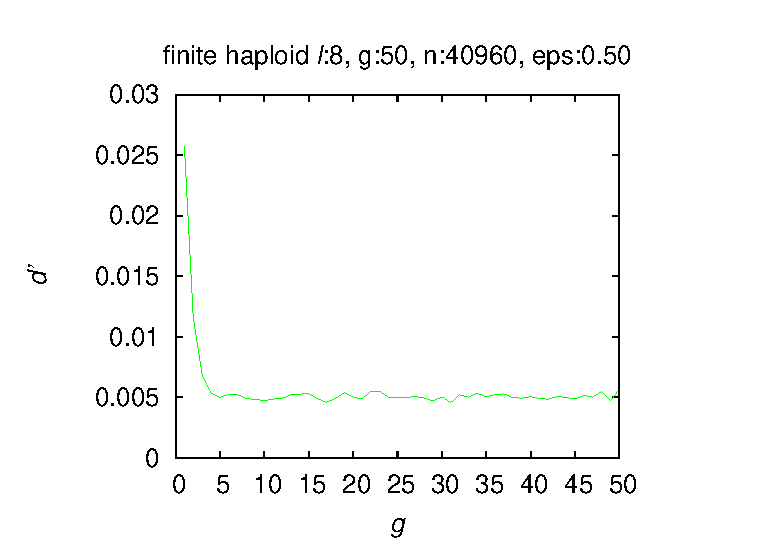
\includegraphics{figures/eps/vio/mu/b8/e0.5/n00040960_fin_hap.eps}}}  \hspace{-3em}%
\subfloat{
\resizebox{8cm}{5cm}{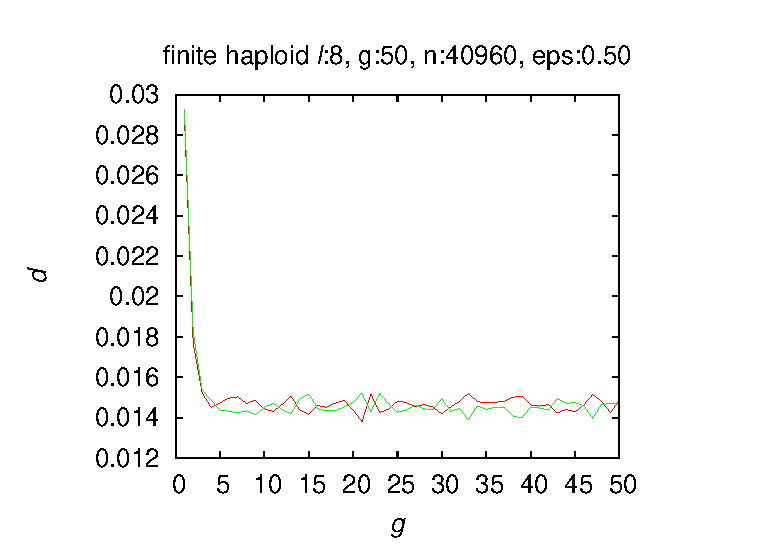
\includegraphics{figures/eps/vio/mu/b8/e0.5/n00040960_fin_hap_wovio.eps}}}\vspace{-1em}  \hspace{-3em}%
\end{center}

\begin{center}
\subfloat{
\resizebox{8cm}{5cm}{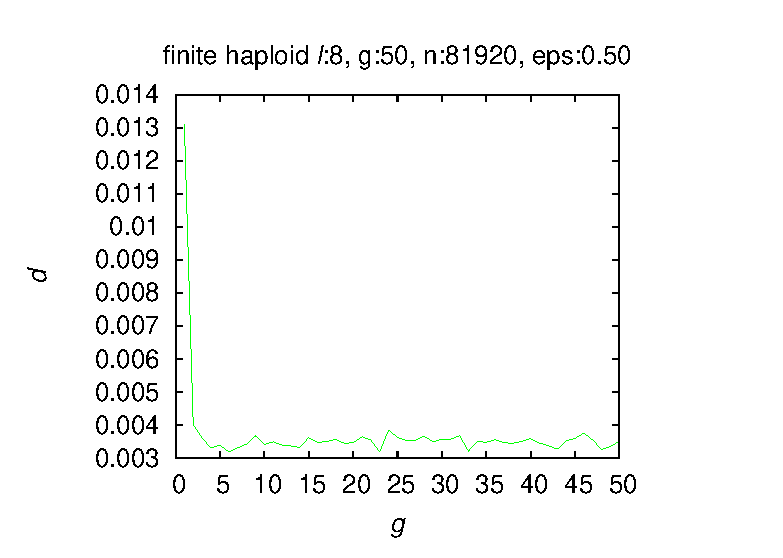
\includegraphics{figures/eps/vio/mu/b8/e0.5/n00081920_fin_hap.eps}}}  \hspace{-3em}%
\subfloat{
\resizebox{8cm}{5cm}{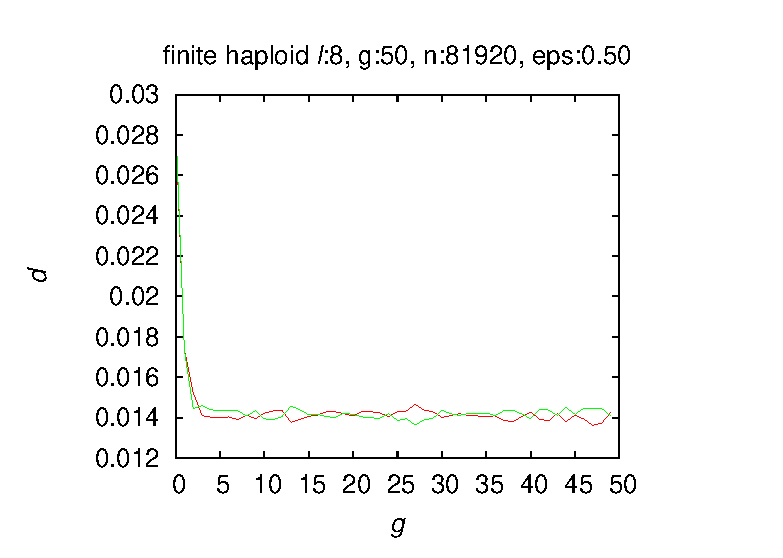
\includegraphics{figures/eps/vio/mu/b8/e0.5/n00081920_fin_hap_wovio.eps}}}\vspace{-1em}  \hspace{-3em}%
\end{center}

\begin{center}
\subfloat{
\resizebox{8cm}{5cm}{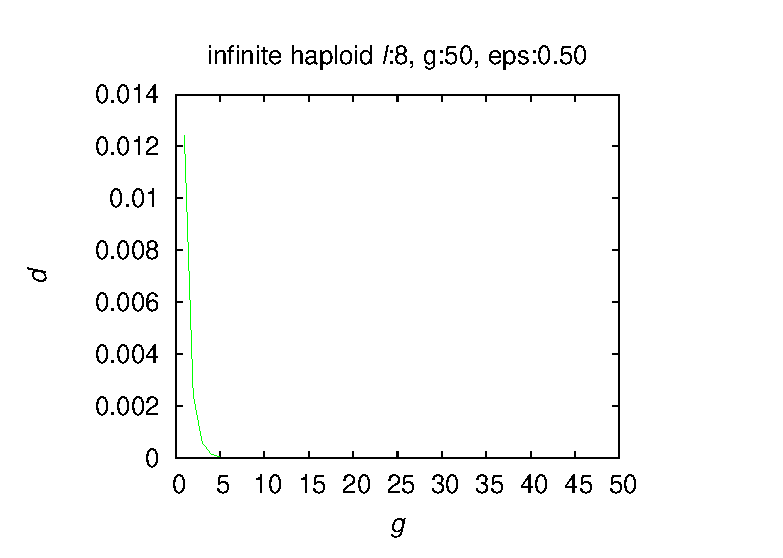
\includegraphics{figures/eps/vio/mu/b8/e0.5/inf_hap.eps}}} \hspace{-3em}%
\subfloat{
\resizebox{8cm}{5cm}{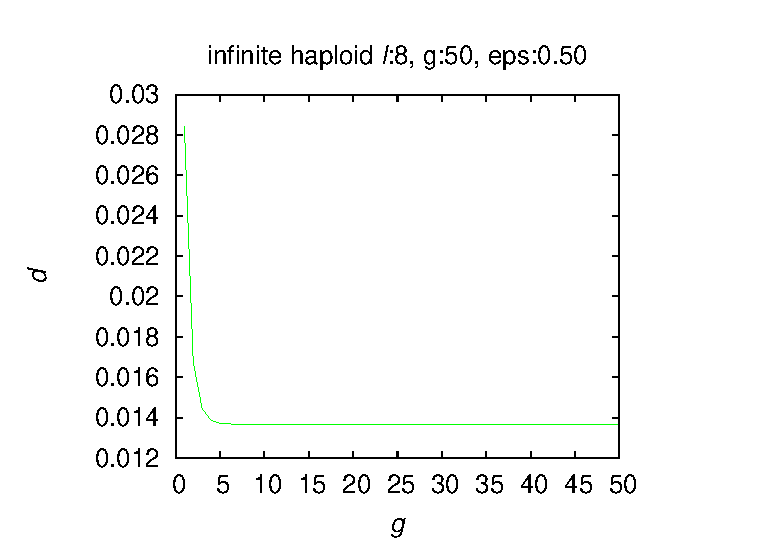
\includegraphics{figures/eps/vio/mu/b8/e0.5/inf_hap_wovio.eps}}}\vspace{-0.5em}  \hspace{-3em}%


\caption{\textbf{Infinite and finite haploid population oscillation behavior in case of violation in $\bm{\mu}$ for 
  genome length $\ell = 8$ and $\epsilon = 0.5$:} In left column, $d$ is distance of finite population of size $n$ or infinite population to limit for $g$ generations. In right column, $d$ is distance of finite population of size $N$ or infinite population to limits without violation.}
\label{oscillation_8h_vio_mu_0.5}
\end{center}
\end{figure}


% l = 10

\begin{figure}[H]
\begin{center}
\subfloat{
\resizebox{8cm}{5cm}{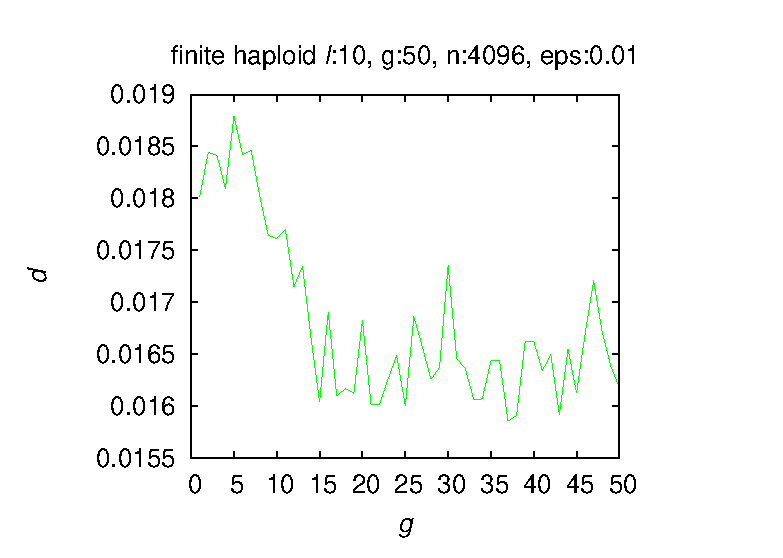
\includegraphics{figures/eps/vio/mu/b10/e0.01/n00004096_fin_hap.eps}}} \hspace{-3em}%
\subfloat{
\resizebox{8cm}{5cm}{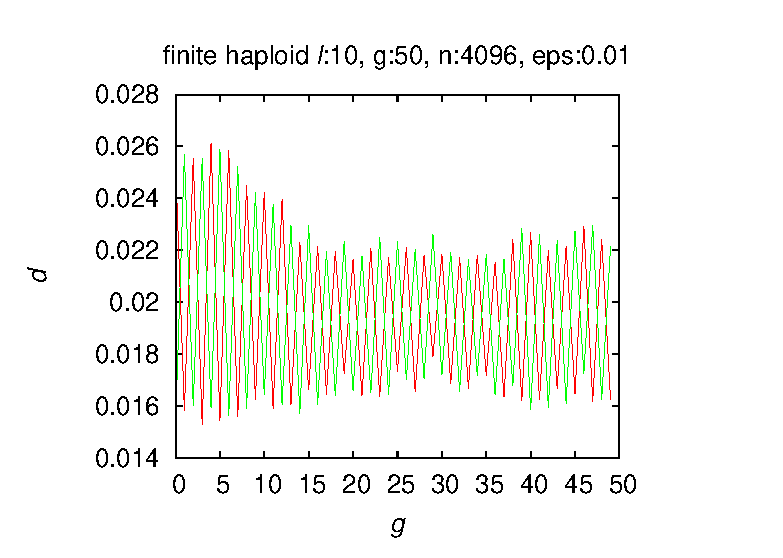
\includegraphics{figures/eps/vio/mu/b10/e0.01/n00004096_fin_hap_wovio.eps}}}\vspace{-1em} \hspace{-3em}%
\end{center}
\begin{center}
\subfloat{
\resizebox{8cm}{5cm}{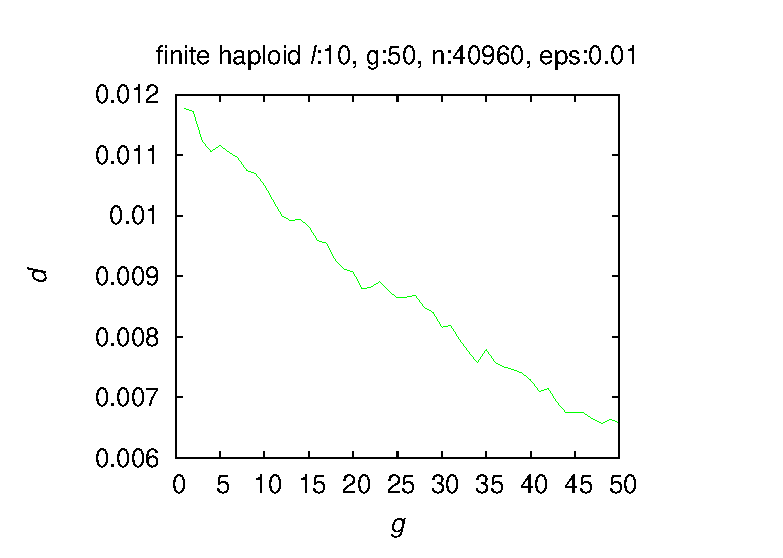
\includegraphics{figures/eps/vio/mu/b10/e0.01/n00040960_fin_hap.eps}}} \hspace{-3em}%
\subfloat{
\resizebox{8cm}{5cm}{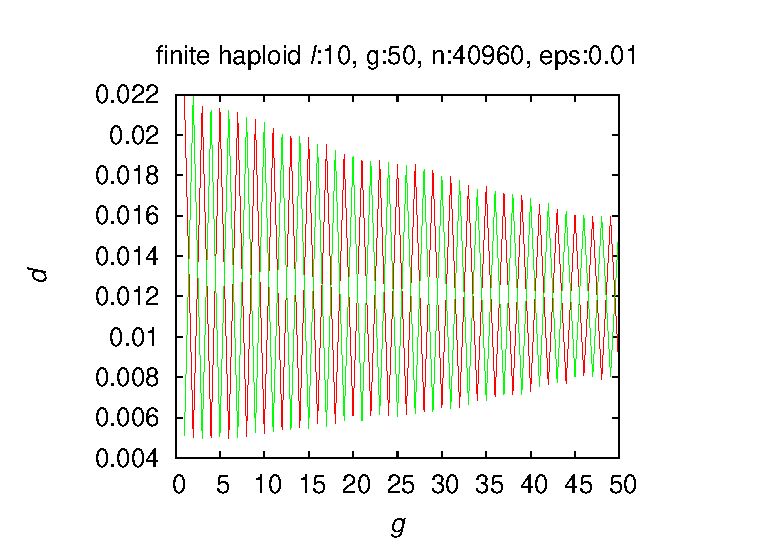
\includegraphics{figures/eps/vio/mu/b10/e0.01/n00040960_fin_hap_wovio.eps}}}\vspace{-1em} \hspace{-3em}%
\end{center}

\begin{center}
\subfloat{
\resizebox{8cm}{5cm}{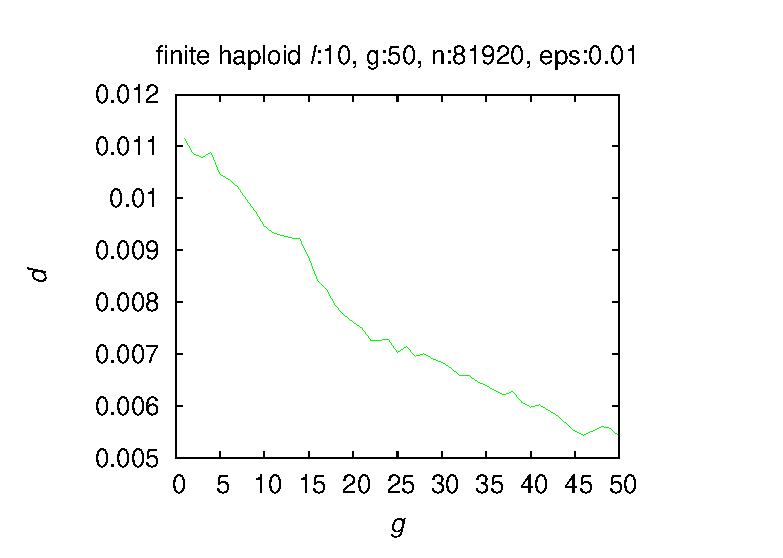
\includegraphics{figures/eps/vio/mu/b10/e0.01/n00081920_fin_hap.eps}}} \hspace{-3em}%
\subfloat{
\resizebox{8cm}{5cm}{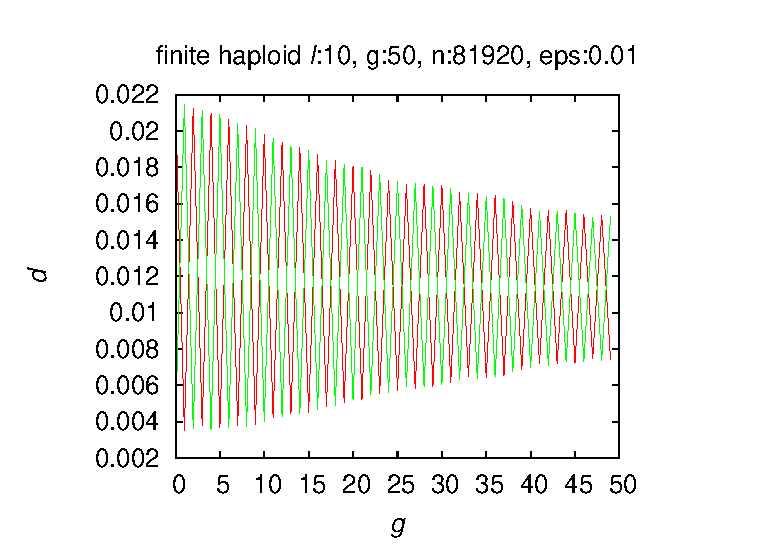
\includegraphics{figures/eps/vio/mu/b10/e0.01/n00081920_fin_hap_wovio.eps}}}\vspace{-1em} \hspace{-3em}%
\end{center}

\begin{center}
\subfloat{
\resizebox{8cm}{5cm}{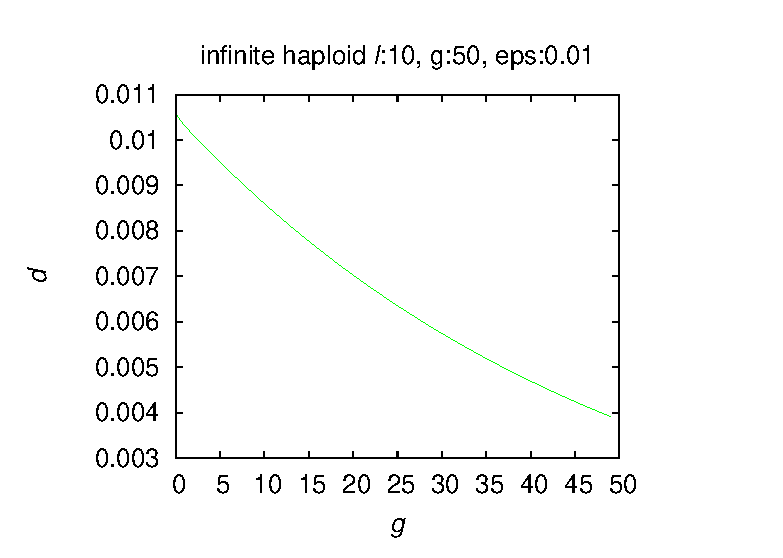
\includegraphics{figures/eps/vio/mu/b10/e0.01/inf_hap.eps}}}\hspace{-3em}%
\subfloat{
\resizebox{8cm}{5cm}{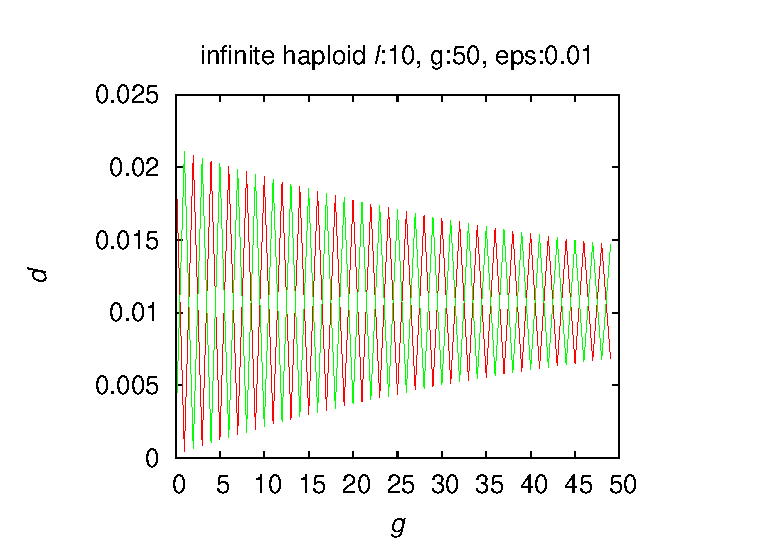
\includegraphics{figures/eps/vio/mu/b10/e0.01/inf_hap_wovio.eps}}}\vspace{-0.5em} \hspace{-3em}%


\caption{\textbf{Infinite and finite haploid population oscillation behavior in case of violation in $\bm{\mu}$ for genome length $\ell = 10$ and $\epsilon = 0.01$:} 
  In left column, $d$ is distance of finite population of size $n$ or infinite population to limit for $g$ generations. In right column, $d$ is distance of finite population of size $N$ or infinite population to limits without violation.}
\label{oscillation_10h_vio_mu_0.01}
\end{center}
\end{figure}



\begin{figure}[H]
\begin{center}
\subfloat{
\resizebox{8cm}{5cm}{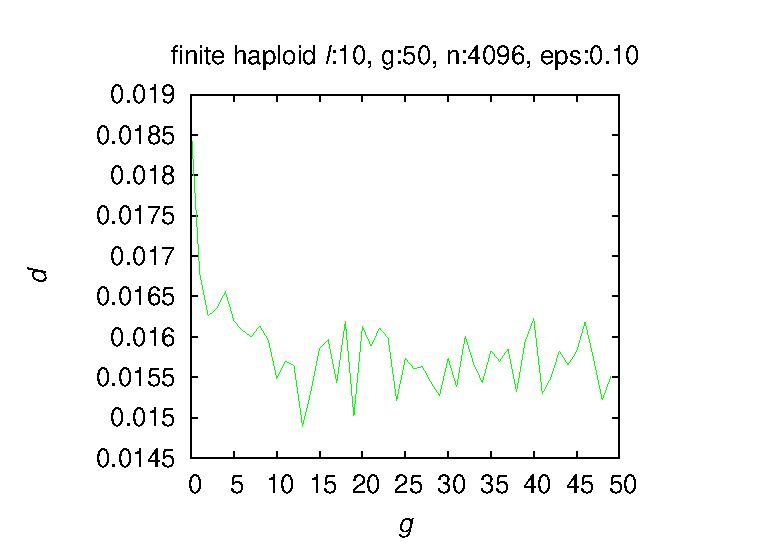
\includegraphics{figures/eps/vio/mu/b10/e0.1/n00004096_fin_hap.eps}}}  \hspace{-3em}%
\subfloat{
\resizebox{8cm}{5cm}{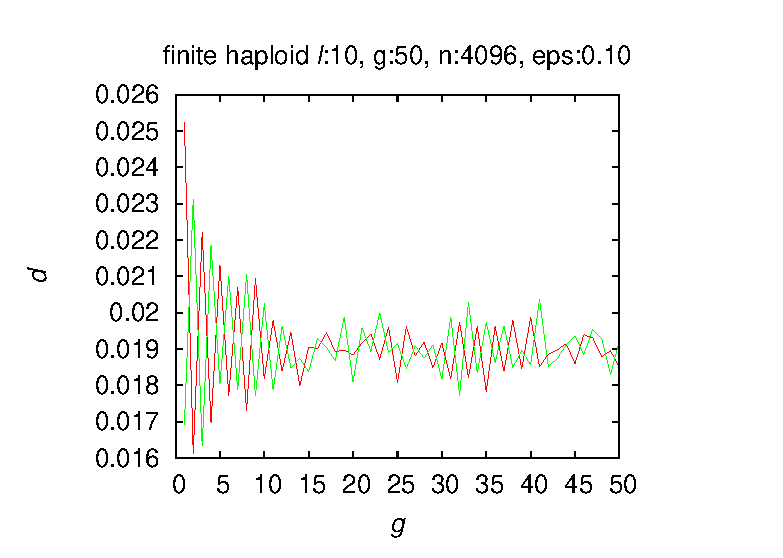
\includegraphics{figures/eps/vio/mu/b10/e0.1/n00004096_fin_hap_wovio.eps}}}\vspace{-1em}  \hspace{-3em}%
\end{center}
\begin{center}
\subfloat{
\resizebox{8cm}{5cm}{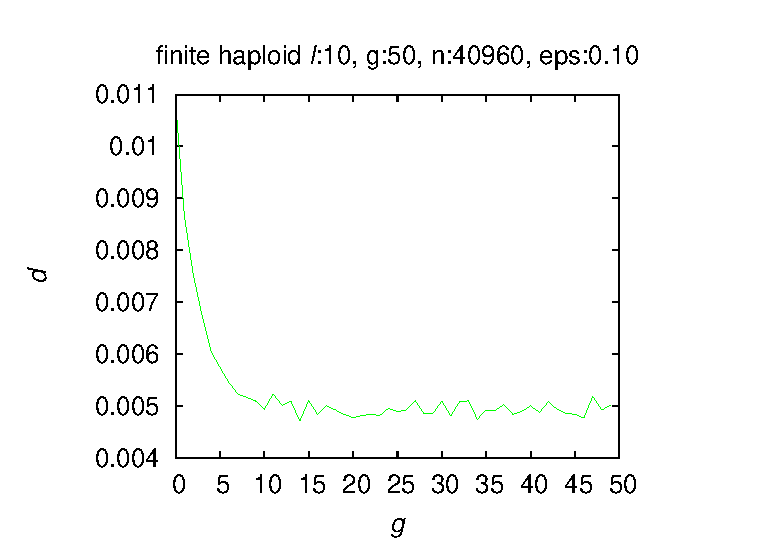
\includegraphics{figures/eps/vio/mu/b10/e0.1/n00040960_fin_hap.eps}}}  \hspace{-3em}%
\subfloat{
\resizebox{8cm}{5cm}{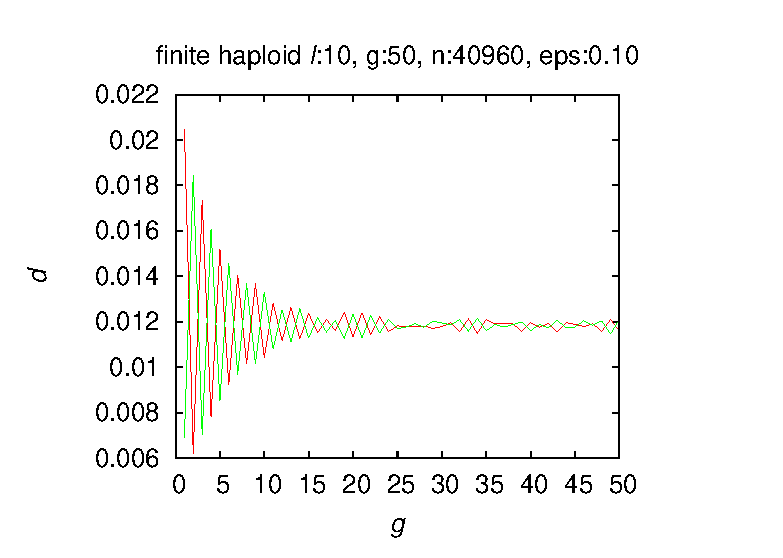
\includegraphics{figures/eps/vio/mu/b10/e0.1/n00040960_fin_hap_wovio.eps}}}\vspace{-1em}  \hspace{-3em}%
\end{center}

\begin{center}
\subfloat{
\resizebox{8cm}{5cm}{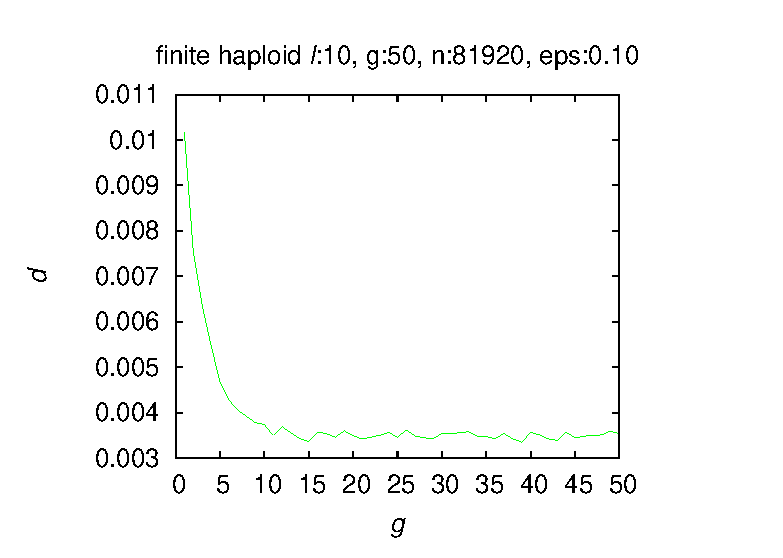
\includegraphics{figures/eps/vio/mu/b10/e0.1/n00081920_fin_hap.eps}}}  \hspace{-3em}%
\subfloat{
\resizebox{8cm}{5cm}{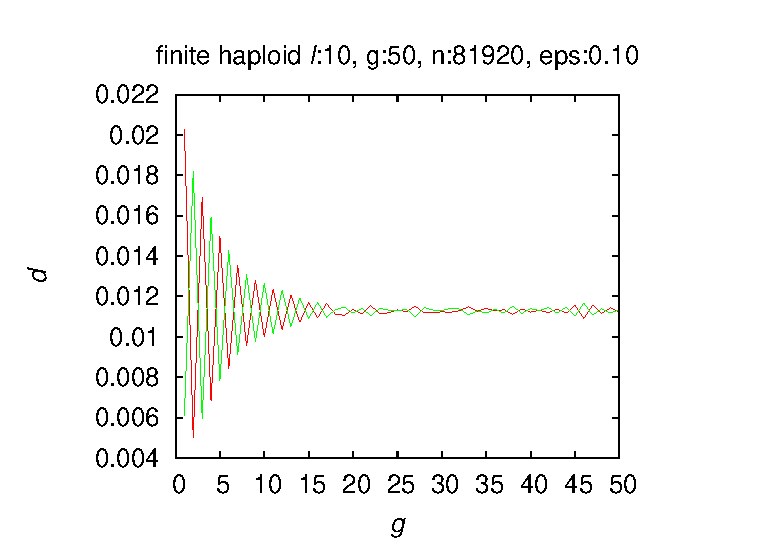
\includegraphics{figures/eps/vio/mu/b10/e0.1/n00081920_fin_hap_wovio.eps}}}\vspace{-1em}  \hspace{-3em}%
\end{center}

\begin{center}
\subfloat{
\resizebox{8cm}{5cm}{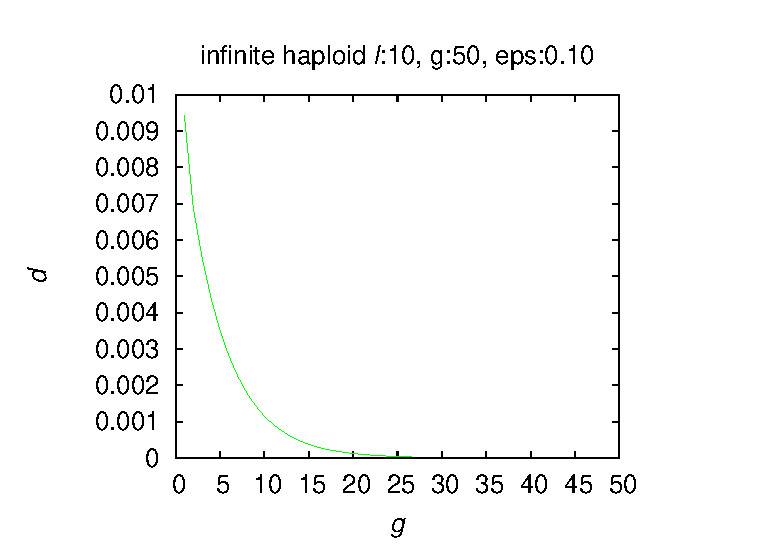
\includegraphics{figures/eps/vio/mu/b10/e0.1/inf_hap.eps}}} \hspace{-3em}%
\subfloat{
\resizebox{8cm}{5cm}{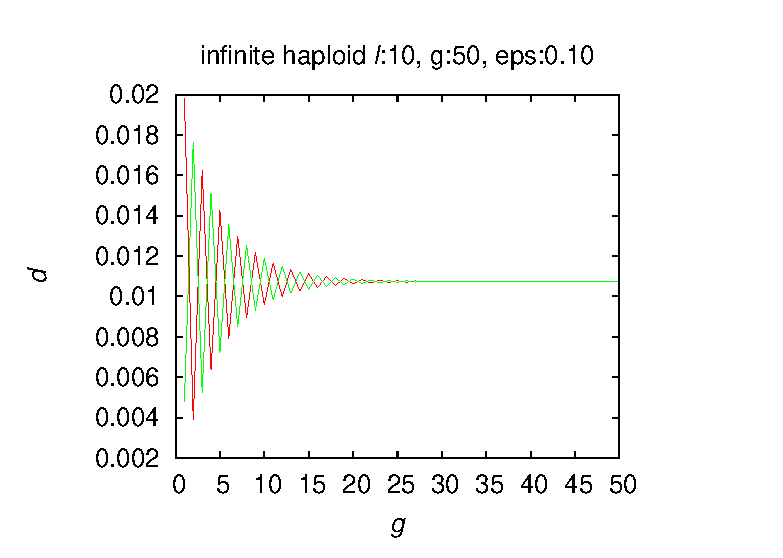
\includegraphics{figures/eps/vio/mu/b10/e0.1/inf_hap_wovio.eps}}}\vspace{-0.5em}  \hspace{-3em}%


\caption{\textbf{Infinite and finite haploid population oscillation behavior in case of violation in $\bm{\mu}$ for genome length $\ell = 10$ and $\epsilon = 0.1$:} 
  In left column, $d$ is distance of finite population of size $n$ or infinite population to limit for $g$ generations. In right column, $d$ is distance of finite population of size $N$ or infinite population to limits without violation.}
\label{oscillation_10h_vio_mu_0.1}
\end{center}
\end{figure}


\begin{figure}[H]

\begin{center}
\subfloat{
\resizebox{8cm}{5cm}{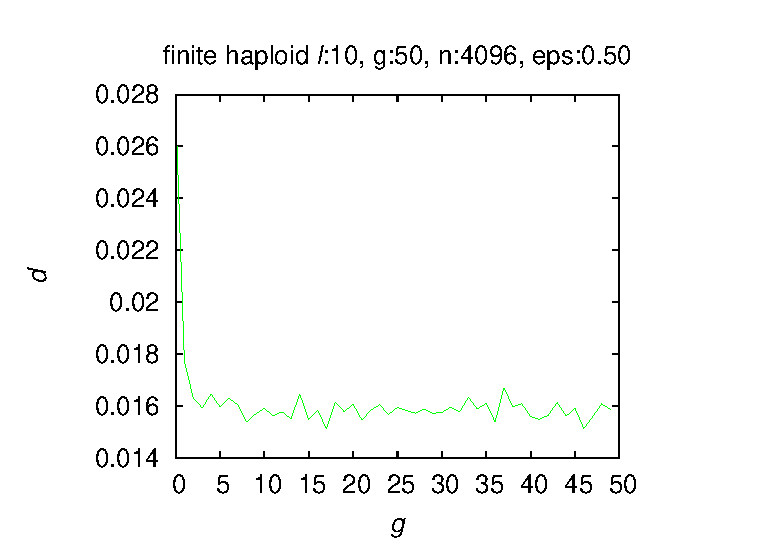
\includegraphics{figures/eps/vio/mu/b10/e0.5/n00004096_fin_hap.eps}}}  \hspace{-3em}%
\subfloat{
\resizebox{8cm}{5cm}{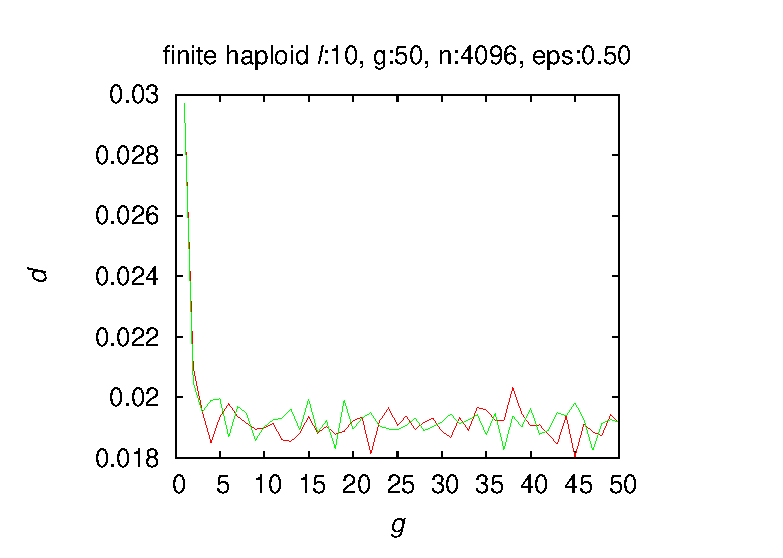
\includegraphics{figures/eps/vio/mu/b10/e0.5/n00004096_fin_hap_wovio.eps}}}\vspace{-1em}  \hspace{-3em}%
\end{center}
\begin{center}
\subfloat{
\resizebox{8cm}{5cm}{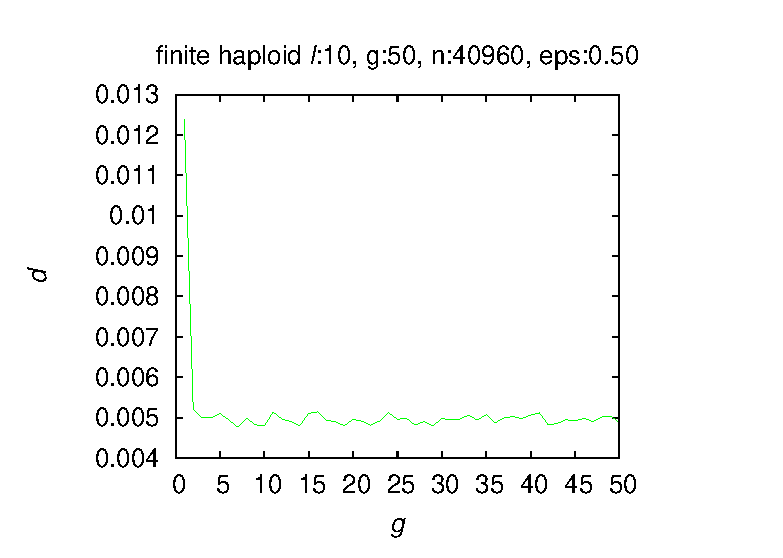
\includegraphics{figures/eps/vio/mu/b10/e0.5/n00040960_fin_hap.eps}}}  \hspace{-3em}%
\subfloat{
\resizebox{8cm}{5cm}{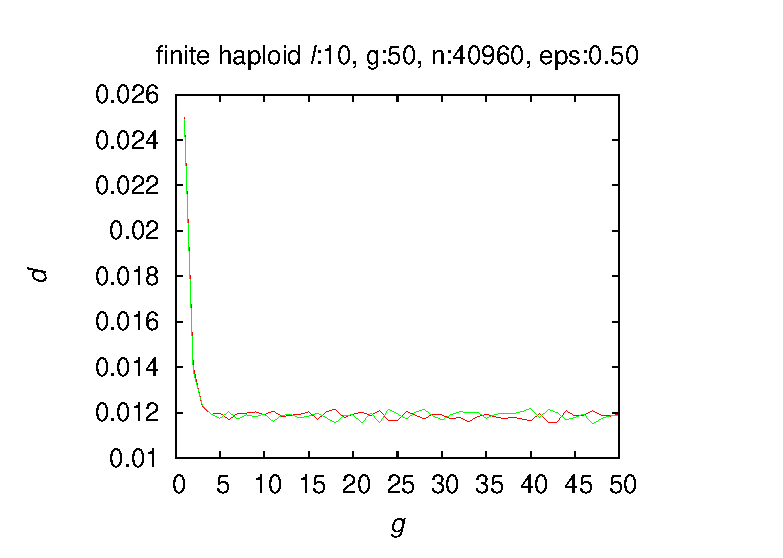
\includegraphics{figures/eps/vio/mu/b10/e0.5/n00040960_fin_hap_wovio.eps}}}\vspace{-1em}  \hspace{-3em}%
\end{center}

\begin{center}
\subfloat{
\resizebox{8cm}{5cm}{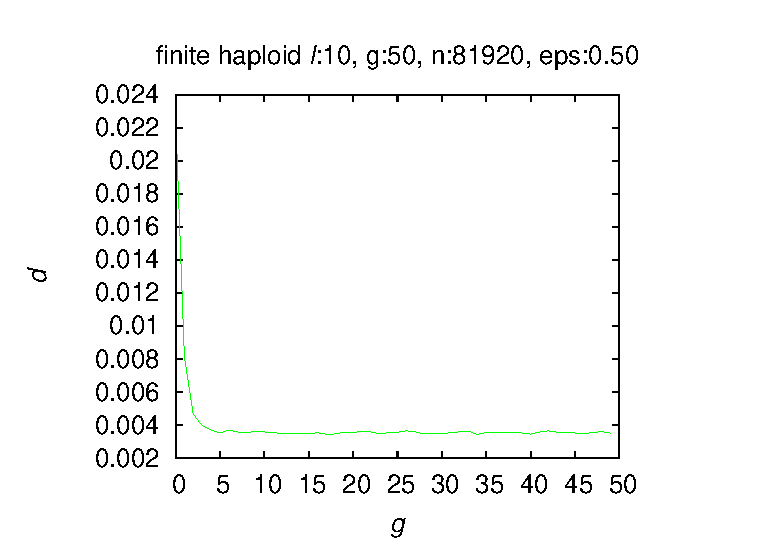
\includegraphics{figures/eps/vio/mu/b10/e0.5/n00081920_fin_hap.eps}}}  \hspace{-3em}%
\subfloat{
\resizebox{8cm}{5cm}{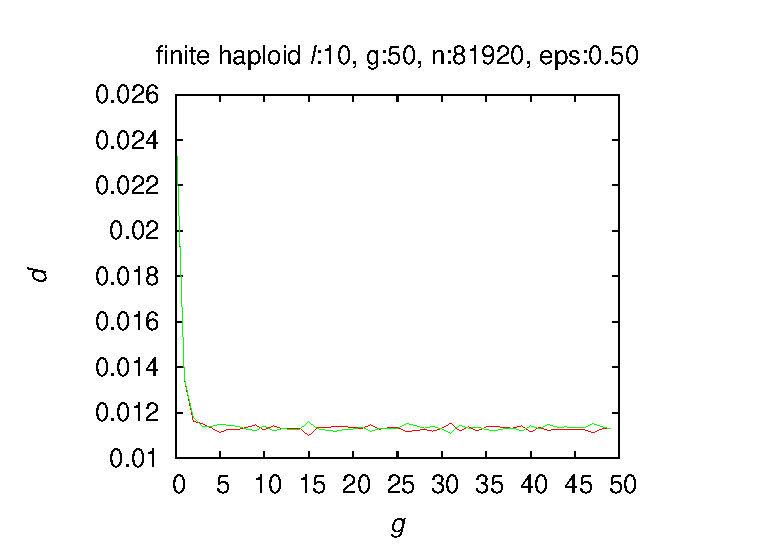
\includegraphics{figures/eps/vio/mu/b10/e0.5/n00081920_fin_hap_wovio.eps}}}\vspace{-1em}  \hspace{-3em}%
\end{center}

\begin{center}
\subfloat{
\resizebox{8cm}{5cm}{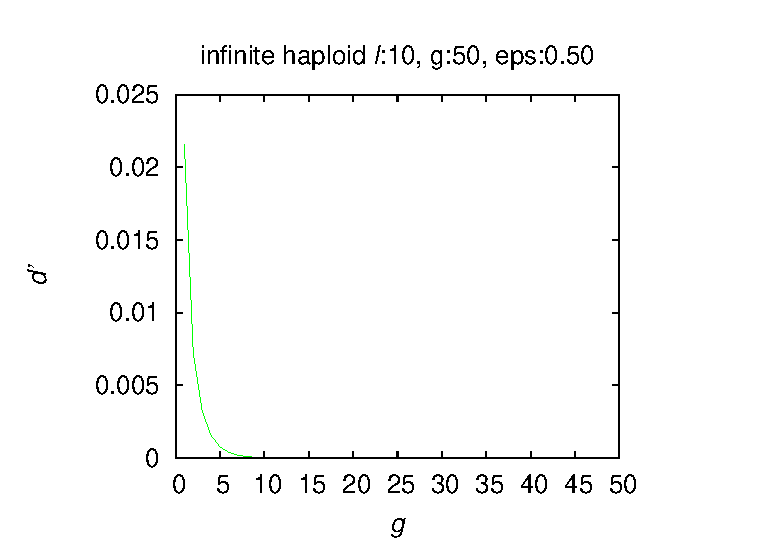
\includegraphics{figures/eps/vio/mu/b10/e0.5/inf_hap.eps}}} \hspace{-3em}%
\subfloat{
\resizebox{8cm}{5cm}{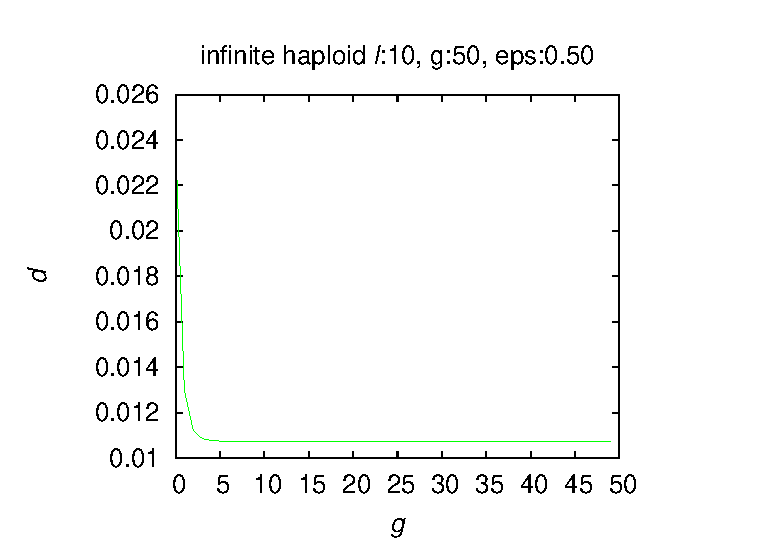
\includegraphics{figures/eps/vio/mu/b10/e0.5/inf_hap_wovio.eps}}}\vspace{-0.5em}  \hspace{-3em}%


\caption{\textbf{Infinite and finite haploid population oscillation behavior in case of violation in $\bm{\mu}$ for 
  genome length $\ell = 10$ and $\epsilon = 0.5$:} In left column, $d$ is distance of finite population of size $n$ or infinite population to limit for $g$ generations. In right column, $d$ is distance of finite population of size $N$ or infinite population to limits without violation.}
\label{oscillation_10h_vio_mu_0.5}
\end{center}
\end{figure}


\begin{figure}[H]
\begin{center}
\subfloat{
\resizebox{8cm}{5cm}{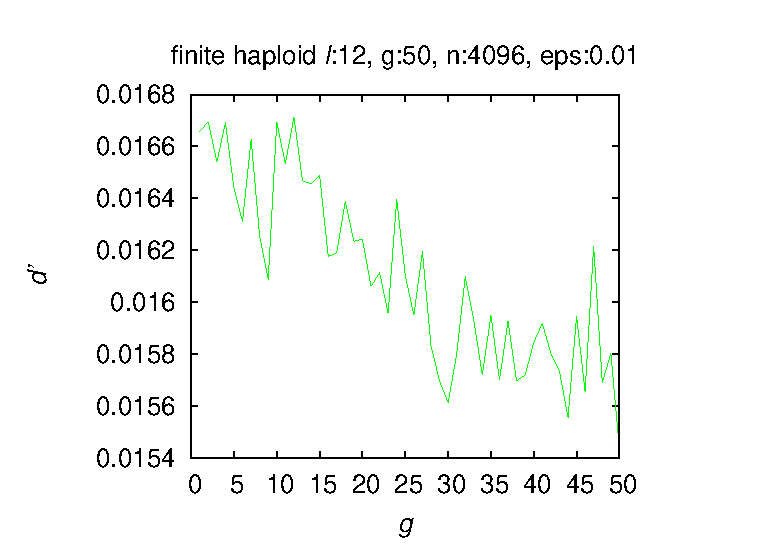
\includegraphics{figures/eps/vio/mu/b12/e0.01/n00004096_fin_hap.eps}}} \hspace{-3em}%
\subfloat{
\resizebox{8cm}{5cm}{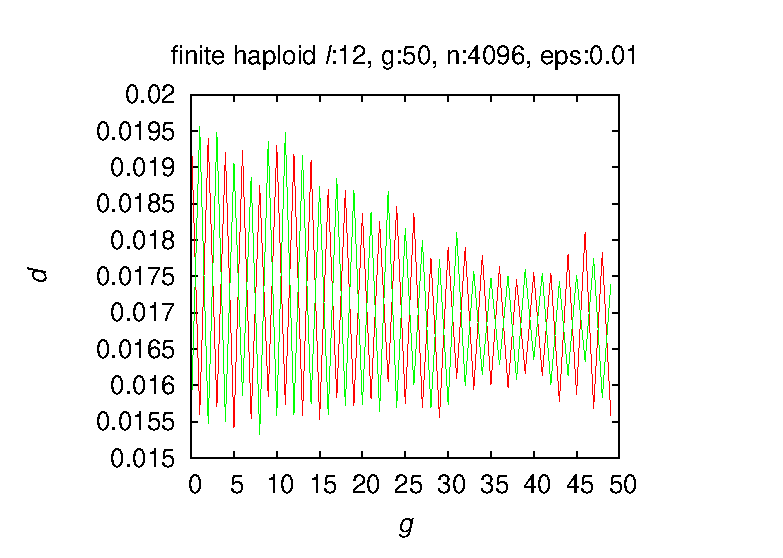
\includegraphics{figures/eps/vio/mu/b12/e0.01/n00004096_fin_hap_wovio.eps}}}\vspace{-1em} \hspace{-3em}%
\end{center}
\begin{center}
\subfloat{
\resizebox{8cm}{5cm}{\includegraphics{figures/eps/vio/mu/b12/e0.01/n00040960_fin_hap.eps}}} \hspace{-3em}%
\subfloat{
\resizebox{8cm}{5cm}{\includegraphics{figures/eps/vio/mu/b12/e0.01/n00040960_fin_hap_wovio.eps}}}\vspace{-1em} \hspace{-3em}%
\end{center}

\begin{center}
\subfloat{
\resizebox{8cm}{5cm}{\includegraphics{figures/eps/vio/mu/b12/e0.01/n00081920_fin_hap.eps}}} \hspace{-3em}%
\subfloat{
\resizebox{8cm}{5cm}{\includegraphics{figures/eps/vio/mu/b12/e0.01/n00081920_fin_hap_wovio.eps}}}\vspace{-1em} \hspace{-3em}%
\end{center}

\begin{center}
\subfloat{
\resizebox{8cm}{5cm}{\includegraphics{figures/eps/vio/mu/b12/e0.01/inf_hap.eps}}}\hspace{-3em}%
\subfloat{
\resizebox{8cm}{5cm}{\includegraphics{figures/eps/vio/mu/b12/e0.01/inf_hap_wovio.eps}}}\vspace{-0.5em} \hspace{-3em}%


\caption{\textbf{Infinite and finite haploid population oscillation behavior in case of violation in $\bm{\mu}$ for genome length $\ell = 12$ and $\epsilon = 0.01$:} 
  In left column, $d$ is distance of finite population of size $n$ or infinite population to limit for $g$ generations. In right column, $d$ is distance of finite population of size $N$ or infinite population to limits without violation.}
\label{oscillation_12h_vio_mu_0.01}
\end{center}
\end{figure}


\begin{figure}[H]
\begin{center}
\subfloat{
\resizebox{8cm}{5cm}{\includegraphics{figures/eps/vio/mu/b12/e0.1/n00004096_fin_hap.eps}}}  \hspace{-3em}%
\subfloat{
\resizebox{8cm}{5cm}{\includegraphics{figures/eps/vio/mu/b12/e0.1/n00004096_fin_hap_wovio.eps}}}\vspace{-1em}  \hspace{-3em}%
\end{center}
\begin{center}
\subfloat{
\resizebox{8cm}{5cm}{\includegraphics{figures/eps/vio/mu/b12/e0.1/n00040960_fin_hap.eps}}}  \hspace{-3em}%
\subfloat{
\resizebox{8cm}{5cm}{\includegraphics{figures/eps/vio/mu/b12/e0.1/n00040960_fin_hap_wovio.eps}}}\vspace{-1em}  \hspace{-3em}%
\end{center}

\begin{center}
\subfloat{
\resizebox{8cm}{5cm}{\includegraphics{figures/eps/vio/mu/b12/e0.1/n00081920_fin_hap.eps}}}  \hspace{-3em}%
\subfloat{
\resizebox{8cm}{5cm}{\includegraphics{figures/eps/vio/mu/b12/e0.1/n00081920_fin_hap_wovio.eps}}}\vspace{-1em}  \hspace{-3em}%
\end{center}

\begin{center}
\subfloat{
\resizebox{8cm}{5cm}{\includegraphics{figures/eps/vio/mu/b12/e0.1/inf_hap.eps}}} \hspace{-3em}%
\subfloat{
\resizebox{8cm}{5cm}{\includegraphics{figures/eps/vio/mu/b12/e0.1/inf_hap_wovio.eps}}}\vspace{-0.5em}  \hspace{-3em}%


\caption{\textbf{Infinite and finite haploid population oscillation behavior in case of violation in $\bm{\mu}$ for genome length $\ell = 12$ and $\epsilon = 0.1$:} 
  In left column, $d$ is distance of finite population of size $n$ or infinite population to limit for $g$ generations. In right column, $d$ is distance of finite population of size $N$ or infinite population to limits without violation.}
\label{oscillation_12h_vio_mu_0.1}
\end{center}
\end{figure}

\begin{figure}[H]

\begin{center}
\subfloat{
\resizebox{8cm}{5cm}{\includegraphics{figures/eps/vio/mu/b12/e0.5/n00004096_fin_hap.eps}}}  \hspace{-3em}%
\subfloat{
\resizebox{8cm}{5cm}{\includegraphics{figures/eps/vio/mu/b12/e0.5/n00004096_fin_hap_wovio.eps}}}\vspace{-1em}  \hspace{-3em}%
\end{center}
\begin{center}
\subfloat{
\resizebox{8cm}{5cm}{\includegraphics{figures/eps/vio/mu/b12/e0.5/n00040960_fin_hap.eps}}}  \hspace{-3em}%
\subfloat{
\resizebox{8cm}{5cm}{\includegraphics{figures/eps/vio/mu/b12/e0.5/n00040960_fin_hap_wovio.eps}}}\vspace{-1em}  \hspace{-3em}%
\end{center}

\begin{center}
\subfloat{
\resizebox{8cm}{5cm}{\includegraphics{figures/eps/vio/mu/b12/e0.5/n00081920_fin_hap.eps}}}  \hspace{-3em}%
\subfloat{
\resizebox{8cm}{5cm}{\includegraphics{figures/eps/vio/mu/b12/e0.5/n00081920_fin_hap_wovio.eps}}}\vspace{-1em}  \hspace{-3em}%
\end{center}

\begin{center}
\subfloat{
\resizebox{8cm}{5cm}{\includegraphics{figures/eps/vio/mu/b12/e0.5/inf_hap.eps}}} \hspace{-3em}%
\subfloat{
\resizebox{8cm}{5cm}{\includegraphics{figures/eps/vio/mu/b12/e0.5/inf_hap_wovio.eps}}}\vspace{-0.5em}  \hspace{-3em}%


\caption{\textbf{Infinite and finite haploid population oscillation behavior in case of violation in $\bm{\mu}$ for 
  genome length $\ell = 12$ and $\epsilon = 0.5$:} In left column, $d$ is distance of finite population of size $n$ or infinite population to limit for $g$ generations. In right column, $d$ is distance of finite population of size $N$ or infinite population to limits without violation.}
\label{oscillation_12h_vio_mu_0.5}
\end{center}
\end{figure}


\begin{figure}[H]
\begin{center}
\subfloat{
\resizebox{8cm}{5cm}{\includegraphics{figures/eps/vio/mu/b14/e0.01/n00004096_fin_hap.eps}}} \hspace{-3em}%
\subfloat{
\resizebox{8cm}{5cm}{\includegraphics{figures/eps/vio/mu/b14/e0.01/n00004096_fin_hap_wovio.eps}}}\vspace{-1em} \hspace{-3em}%
\end{center}
\begin{center}
\subfloat{
\resizebox{8cm}{5cm}{\includegraphics{figures/eps/vio/mu/b14/e0.01/n00040960_fin_hap.eps}}} \hspace{-3em}%
\subfloat{
\resizebox{8cm}{5cm}{\includegraphics{figures/eps/vio/mu/b14/e0.01/n00040960_fin_hap_wovio.eps}}}\vspace{-1em} \hspace{-3em}%
\end{center}

\begin{center}
\subfloat{
\resizebox{8cm}{5cm}{\includegraphics{figures/eps/vio/mu/b14/e0.01/n00081920_fin_hap.eps}}} \hspace{-3em}%
\subfloat{
\resizebox{8cm}{5cm}{\includegraphics{figures/eps/vio/mu/b14/e0.01/n00081920_fin_hap_wovio.eps}}}\vspace{-1em} \hspace{-3em}%
\end{center}

\begin{center}
\subfloat{
\resizebox{8cm}{5cm}{\includegraphics{figures/eps/vio/mu/b14/e0.01/inf_hap.eps}}}\hspace{-3em}%
\subfloat{
\resizebox{8cm}{5cm}{\includegraphics{figures/eps/vio/mu/b14/e0.01/inf_hap_wovio.eps}}}\vspace{-0.5em} \hspace{-3em}%


\caption{\textbf{Infinite and finite haploid population oscillation behavior in case of violation in $\bm{\mu}$ for genome length $\ell = 14$ and $\epsilon = 0.01$:} 
  In left column, $d$ is distance of finite population of size $n$ or infinite population to limit for $g$ generations. In right column, $d$ is distance of finite population of size $N$ or infinite population to limits without violation.}
\label{oscillation_14h_vio_mu_0.01}
\end{center}
\end{figure}


\begin{figure}[H]
\begin{center}
\subfloat{
\resizebox{8cm}{5cm}{\includegraphics{figures/eps/vio/mu/b14/e0.1/n00004096_fin_hap.eps}}}  \hspace{-3em}%
\subfloat{
\resizebox{8cm}{5cm}{\includegraphics{figures/eps/vio/mu/b14/e0.1/n00004096_fin_hap_wovio.eps}}}\vspace{-1em}  \hspace{-3em}%
\end{center}
\begin{center}
\subfloat{
\resizebox{8cm}{5cm}{\includegraphics{figures/eps/vio/mu/b14/e0.1/n00040960_fin_hap.eps}}}  \hspace{-3em}%
\subfloat{
\resizebox{8cm}{5cm}{\includegraphics{figures/eps/vio/mu/b14/e0.1/n00040960_fin_hap_wovio.eps}}}\vspace{-1em}  \hspace{-3em}%
\end{center}

\begin{center}
\subfloat{
\resizebox{8cm}{5cm}{\includegraphics{figures/eps/vio/mu/b14/e0.1/n00081920_fin_hap.eps}}}  \hspace{-3em}%
\subfloat{
\resizebox{8cm}{5cm}{\includegraphics{figures/eps/vio/mu/b14/e0.1/n00081920_fin_hap_wovio.eps}}}\vspace{-1em}  \hspace{-3em}%
\end{center}

\begin{center}
\subfloat{
\resizebox{8cm}{5cm}{\includegraphics{figures/eps/vio/mu/b14/e0.1/inf_hap.eps}}} \hspace{-3em}%
\subfloat{
\resizebox{8cm}{5cm}{\includegraphics{figures/eps/vio/mu/b14/e0.1/inf_hap_wovio.eps}}}\vspace{-0.5em}  \hspace{-3em}%


\caption{\textbf{Infinite and finite haploid population oscillation behavior in case of violation in $\bm{\mu}$ for genome length $\ell = 14$ and $\epsilon = 0.1$:} 
  In left column, $d$ is distance of finite population of size $n$ or infinite population to limit for $g$ generations. In right column, $d$ is distance of finite population of size $N$ or infinite population to limits without violation.}
\label{oscillation_14h_vio_mu_0.1}
\end{center}
\end{figure}


\begin{figure}[H]

\begin{center}
\subfloat{
\resizebox{8cm}{5cm}{\includegraphics{figures/eps/vio/mu/b14/e0.5/n00004096_fin_hap.eps}}}  \hspace{-3em}%
\subfloat{
\resizebox{8cm}{5cm}{\includegraphics{figures/eps/vio/mu/b14/e0.5/n00004096_fin_hap_wovio.eps}}}\vspace{-1em}  \hspace{-3em}%
\end{center}
\begin{center}
\subfloat{
\resizebox{8cm}{5cm}{\includegraphics{figures/eps/vio/mu/b14/e0.5/n00040960_fin_hap.eps}}}  \hspace{-3em}%
\subfloat{
\resizebox{8cm}{5cm}{\includegraphics{figures/eps/vio/mu/b14/e0.5/n00040960_fin_hap_wovio.eps}}}\vspace{-1em}  \hspace{-3em}%
\end{center}

\begin{center}
\subfloat{
\resizebox{8cm}{5cm}{\includegraphics{figures/eps/vio/mu/b14/e0.5/n00081920_fin_hap.eps}}}  \hspace{-3em}%
\subfloat{
\resizebox{8cm}{5cm}{\includegraphics{figures/eps/vio/mu/b14/e0.5/n00081920_fin_hap_wovio.eps}}}\vspace{-1em}  \hspace{-3em}%
\end{center}

\begin{center}
\subfloat{
\resizebox{8cm}{5cm}{\includegraphics{figures/eps/vio/mu/b14/e0.5/inf_hap.eps}}} \hspace{-3em}%
\subfloat{
\resizebox{8cm}{5cm}{\includegraphics{figures/eps/vio/mu/b14/e0.5/inf_hap_wovio.eps}}}\vspace{-0.5em}  \hspace{-3em}%


\caption{\textbf{Infinite and finite haploid population oscillation behavior in case of violation in $\bm{\mu}$ for 
  genome length $\ell = 14$ and $\epsilon = 0.5$:} In left column, $d$ is distance of finite population of size $n$ or infinite population to limit for $g$ generations. In right column, $d$ is distance of finite population of size $N$ or infinite population to limits without violation.}
\label{oscillation_14h_vio_mu_0.5}
\end{center}
\end{figure}

